\documentclass[12pt]{article}
\usepackage[a4paper, margin=.30in]{geometry}
\usepackage{graphicx ,
            wrapfig,
            xcolor, 
            enumerate,
            amsmath,fontenc, mhchem
            }

\newcommand\headerMe[2]{\noindent{}#1\hfill#2}
\renewcommand{\thesection}{\Roman{section}}

\author{Zakaria HAOUZAN}
\date{\today}

\begin{document}
% headers --------------
\headerMe{Matière : Physique-Chimie}{Professeur : Zakaria HAOUZAN}\\
\headerMe{Unité : Travail Mécanique et Energie }{Établissement : Lycée SKHOR qualifiant}\\
\headerMe{Niveau : 1BAC-SM-X}{Heure : 6H}\\

% ------Content ________
\begin{center}

    \Large{Leçon $N^{\circ} 6 $: \color{red}Les Réactions d’oxydo-réduction}
\end{center}

%\begin{wrapfigure}[10]{r}{0.5\textwidth}
%    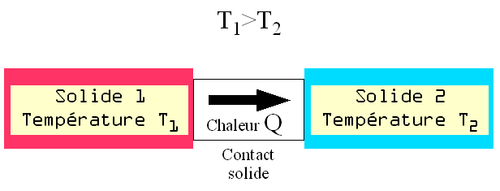
\includegraphics[width=0.5\textwidth]{./img/img00.png}
%\end{wrapfigure}
\section{Notion Réactions d’oxydo-réduction: }
\subsection{Mise en évidence de la notion d’oxydo-réduction :}
\subsubsection{Expérience : }
On immerge partiellement une plaque de cuivre dans un bécher contenant une solution de nitrate d’argent $(Ag^+ + NO_3^-)$

On observe après quelques minutes un dépôt gris sur la partie immergée de la plaque et la solution prend une couleur bleue.

\subsubsection{Interprétation}
L’apparition de la couleur bleue s’explique par la présence des ions $Cu^{2+}$ qui résulte de l’oxydation du cuivre.
La transformation subie par le cuivre métallique Cu(s) se traduit par la demi-équation suivante :
\ce{${\ce{Cu_{}(s)}}$ <=>$\ce{Cu^{2+}_{aq}} + \ce{2e^-}$} 

le couple oxydo-rédox correspondant est $Cu^{2+}/Cu$

On dit que le cuivre Cu a subit une oxydation : donc l’oxydation est une perte d’électrons.
Le dépôt qui se forme sur la plaque est de l’argent métallique $Ag(s)$ qui résulte de la réduction des ions $Ag^+_{(aq)}$
.

La transformation subie par les ions $Ag^+_{(aq)}$se traduit par la demi-équation suivante :
\ce{${\ce{Ag^+_{aq}}} + \ce{1e^-}$ <=>$\ce{Ag_{s}} $} 
On dit que l’ion $Ag^+$ a subi t une réduction : donc la réduction est un gain d’électrons.
On obtient l’équation de la réaction bilan en ajoutant les deux demi-équations précédentes :
\begin{center}

\ce{${\ce{Cu_{}(s)}}$ <=>$\ce{Cu^{2+}_{aq}} + \ce{2e^-}$} 

\ce{${\ce{Ag^+_{aq}}} + \ce{1e^-}$ <=>$\ce{Ag_{s}} $} 

   \ce{${\ce{2Ag^+_{aq}}} + \ce{Cu_{}(s)}$ <=>$\ce{Ag_{s}} + \ce{Cu^{2+}_{aq}} $} 
\end{center}

Remarque : Cette réaction au cours de laquelle il y’a transfert des électrons s’appelle réaction d’oxydo-réduction.
L’espèce qui a subit l’oxydation s’appelle réducteur et l’espèce qui a subit une réduction s’appelle oxydant.
\subsection{Conclusion }
On appelle oxydant toute espèce chimique capable de capter un ou plusieurs électrons au cours d’une réaction chimique.

On appelle réducteur toute espèce chimique capable de perdre un ou plusieurs électrons au cours d’une réaction chimique.

L’oxydation est une perte d’électrons par une espèce chimique (et l’espèce qui a subie l’oxydation s’appelle réducteur)

La réduction est un gain d’électrons par une espèce chimique (et l’espèce qui a subie l La réduction s’appelle oxydant)

Dans le cas général une demi-équation ox/réd s’écrit de la manière suivante :


\ce{\ce{OX} + \ce{$ne^-$} <=>[\text{réduction}][\text{oxydation}] $\ce{red}$}

Remarque : Dans une demi-équation d’oxydo-réduction les électrons se trouvent toujours à coté de l’oxydant.
\end{document}

